\chapter{Perancangan}
\label{chap:perancangan}

Bab ini membahas tentang perancangan untuk implementasi sistem perekaman ulang dalam SharIF-Judge. Perancangan akan dilakukan 

\section{Rancangan Antarmuka}

\subsection{Sistem Rekaman}
\label{sub:4:1:rekaman}

Seluruh sistem rekaman akan diimplementasikan dalam halaman Submit tidak memerlukan perubahan pada antarmuka. Gambar \ref{fig:4:1:submit} menunjukkan halaman Submit dan IDE yang sudah di implementasikan oleh Nicholas Aditya Halim~\cite{nicholas:sharif}.

\begin{figure}[H]
    \centering
    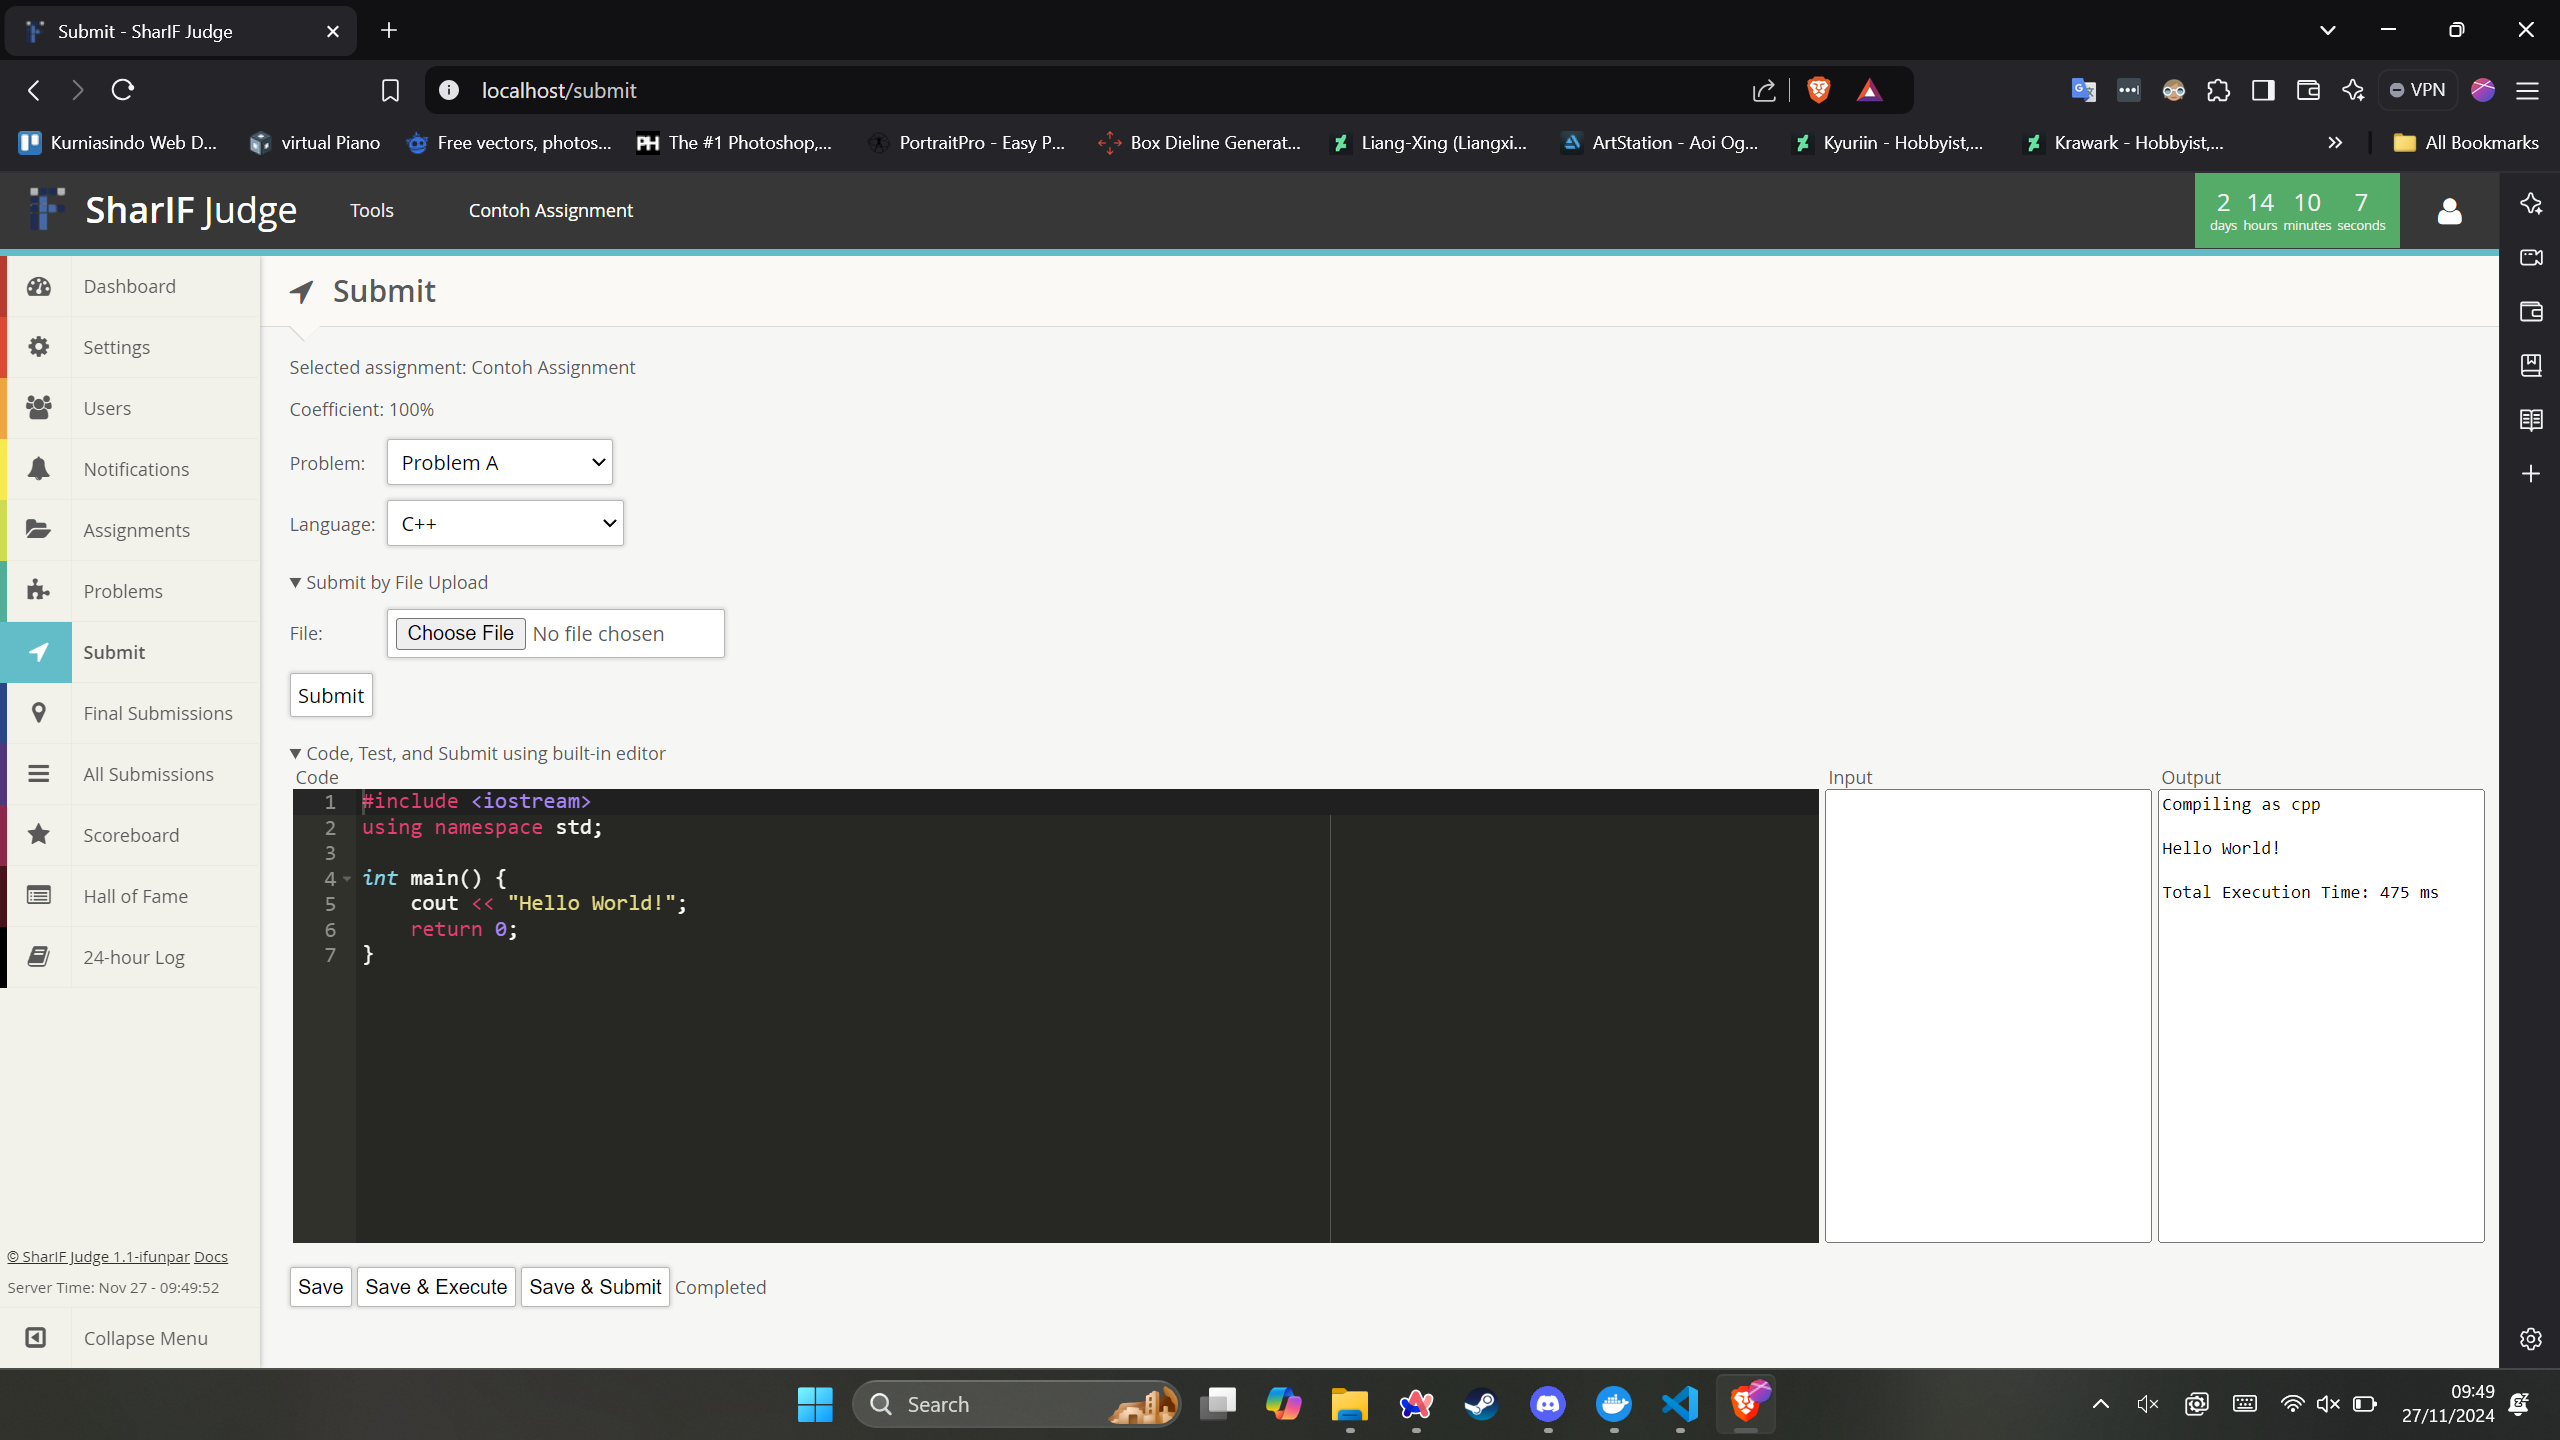
\includegraphics[width=0.75\textwidth]{views/submit.png}
    \caption{Halaman}
    \label{fig:4:1:submit}
\end{figure}

\subsection{Sistem Pemutaran ulang}
\label{sub:4:1:pemutaranulang}

Pada sistem pemutaran ulang dibutuhkan dua halaman baru yaitu halaman untuk menunjukkan daftar rekaman dalam sistem dan halaman untuk sistem pemutaran ulang sebuah rekaman. Gambar \ref{fig:4:1:listrec} merupakan rancangan antarmuka untuk halaman daftar rekaman dan Gambar \ref{fig:4:1:rec} merupakan rancangan antarmuka untuk halaman pemutaran ulang.

\begin{figure}[H]
    \centering
    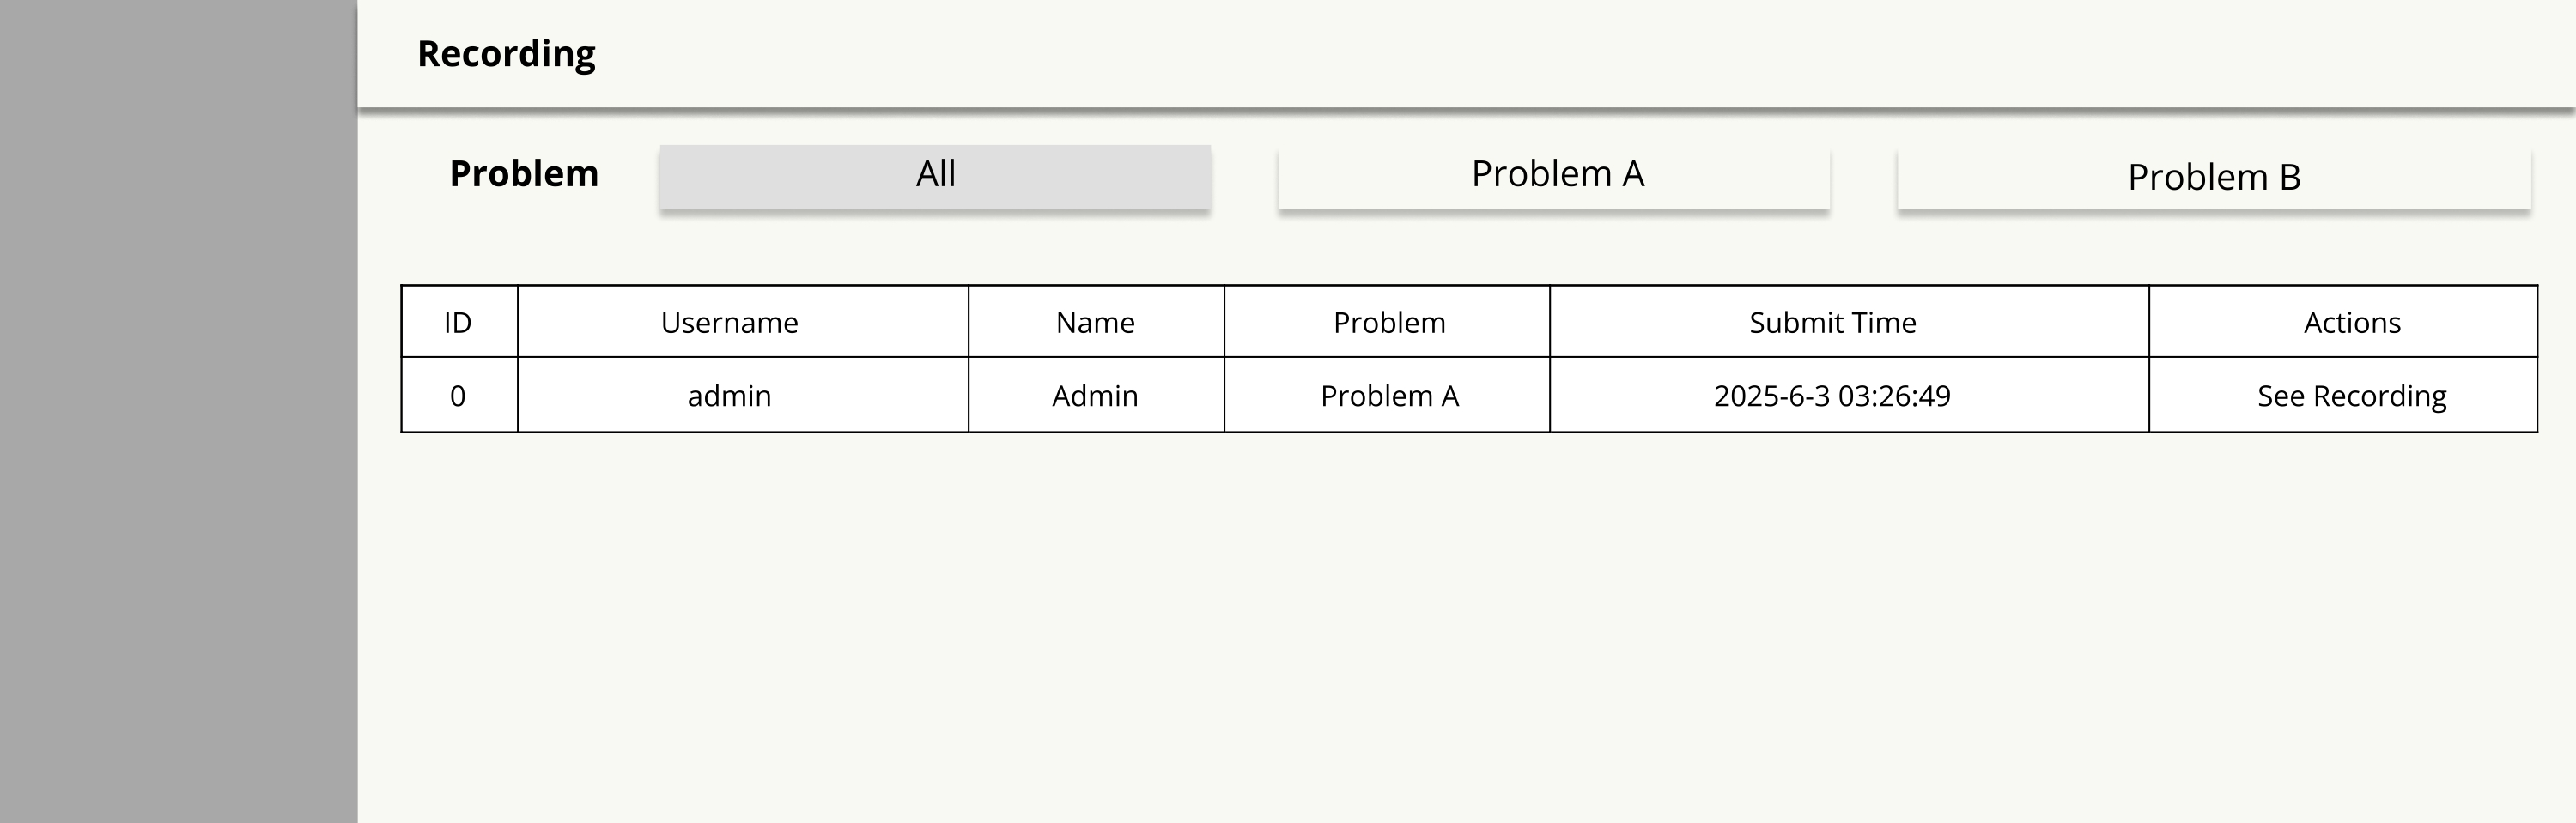
\includegraphics[width=0.75\textwidth]{design-recording-list.jpg}
    \caption{Rancangan Antarmuka Halaman Daftar Rekaman}
    \label{fig:4:1:listrec}
\end{figure}

\begin{figure}[H]
    \centering
    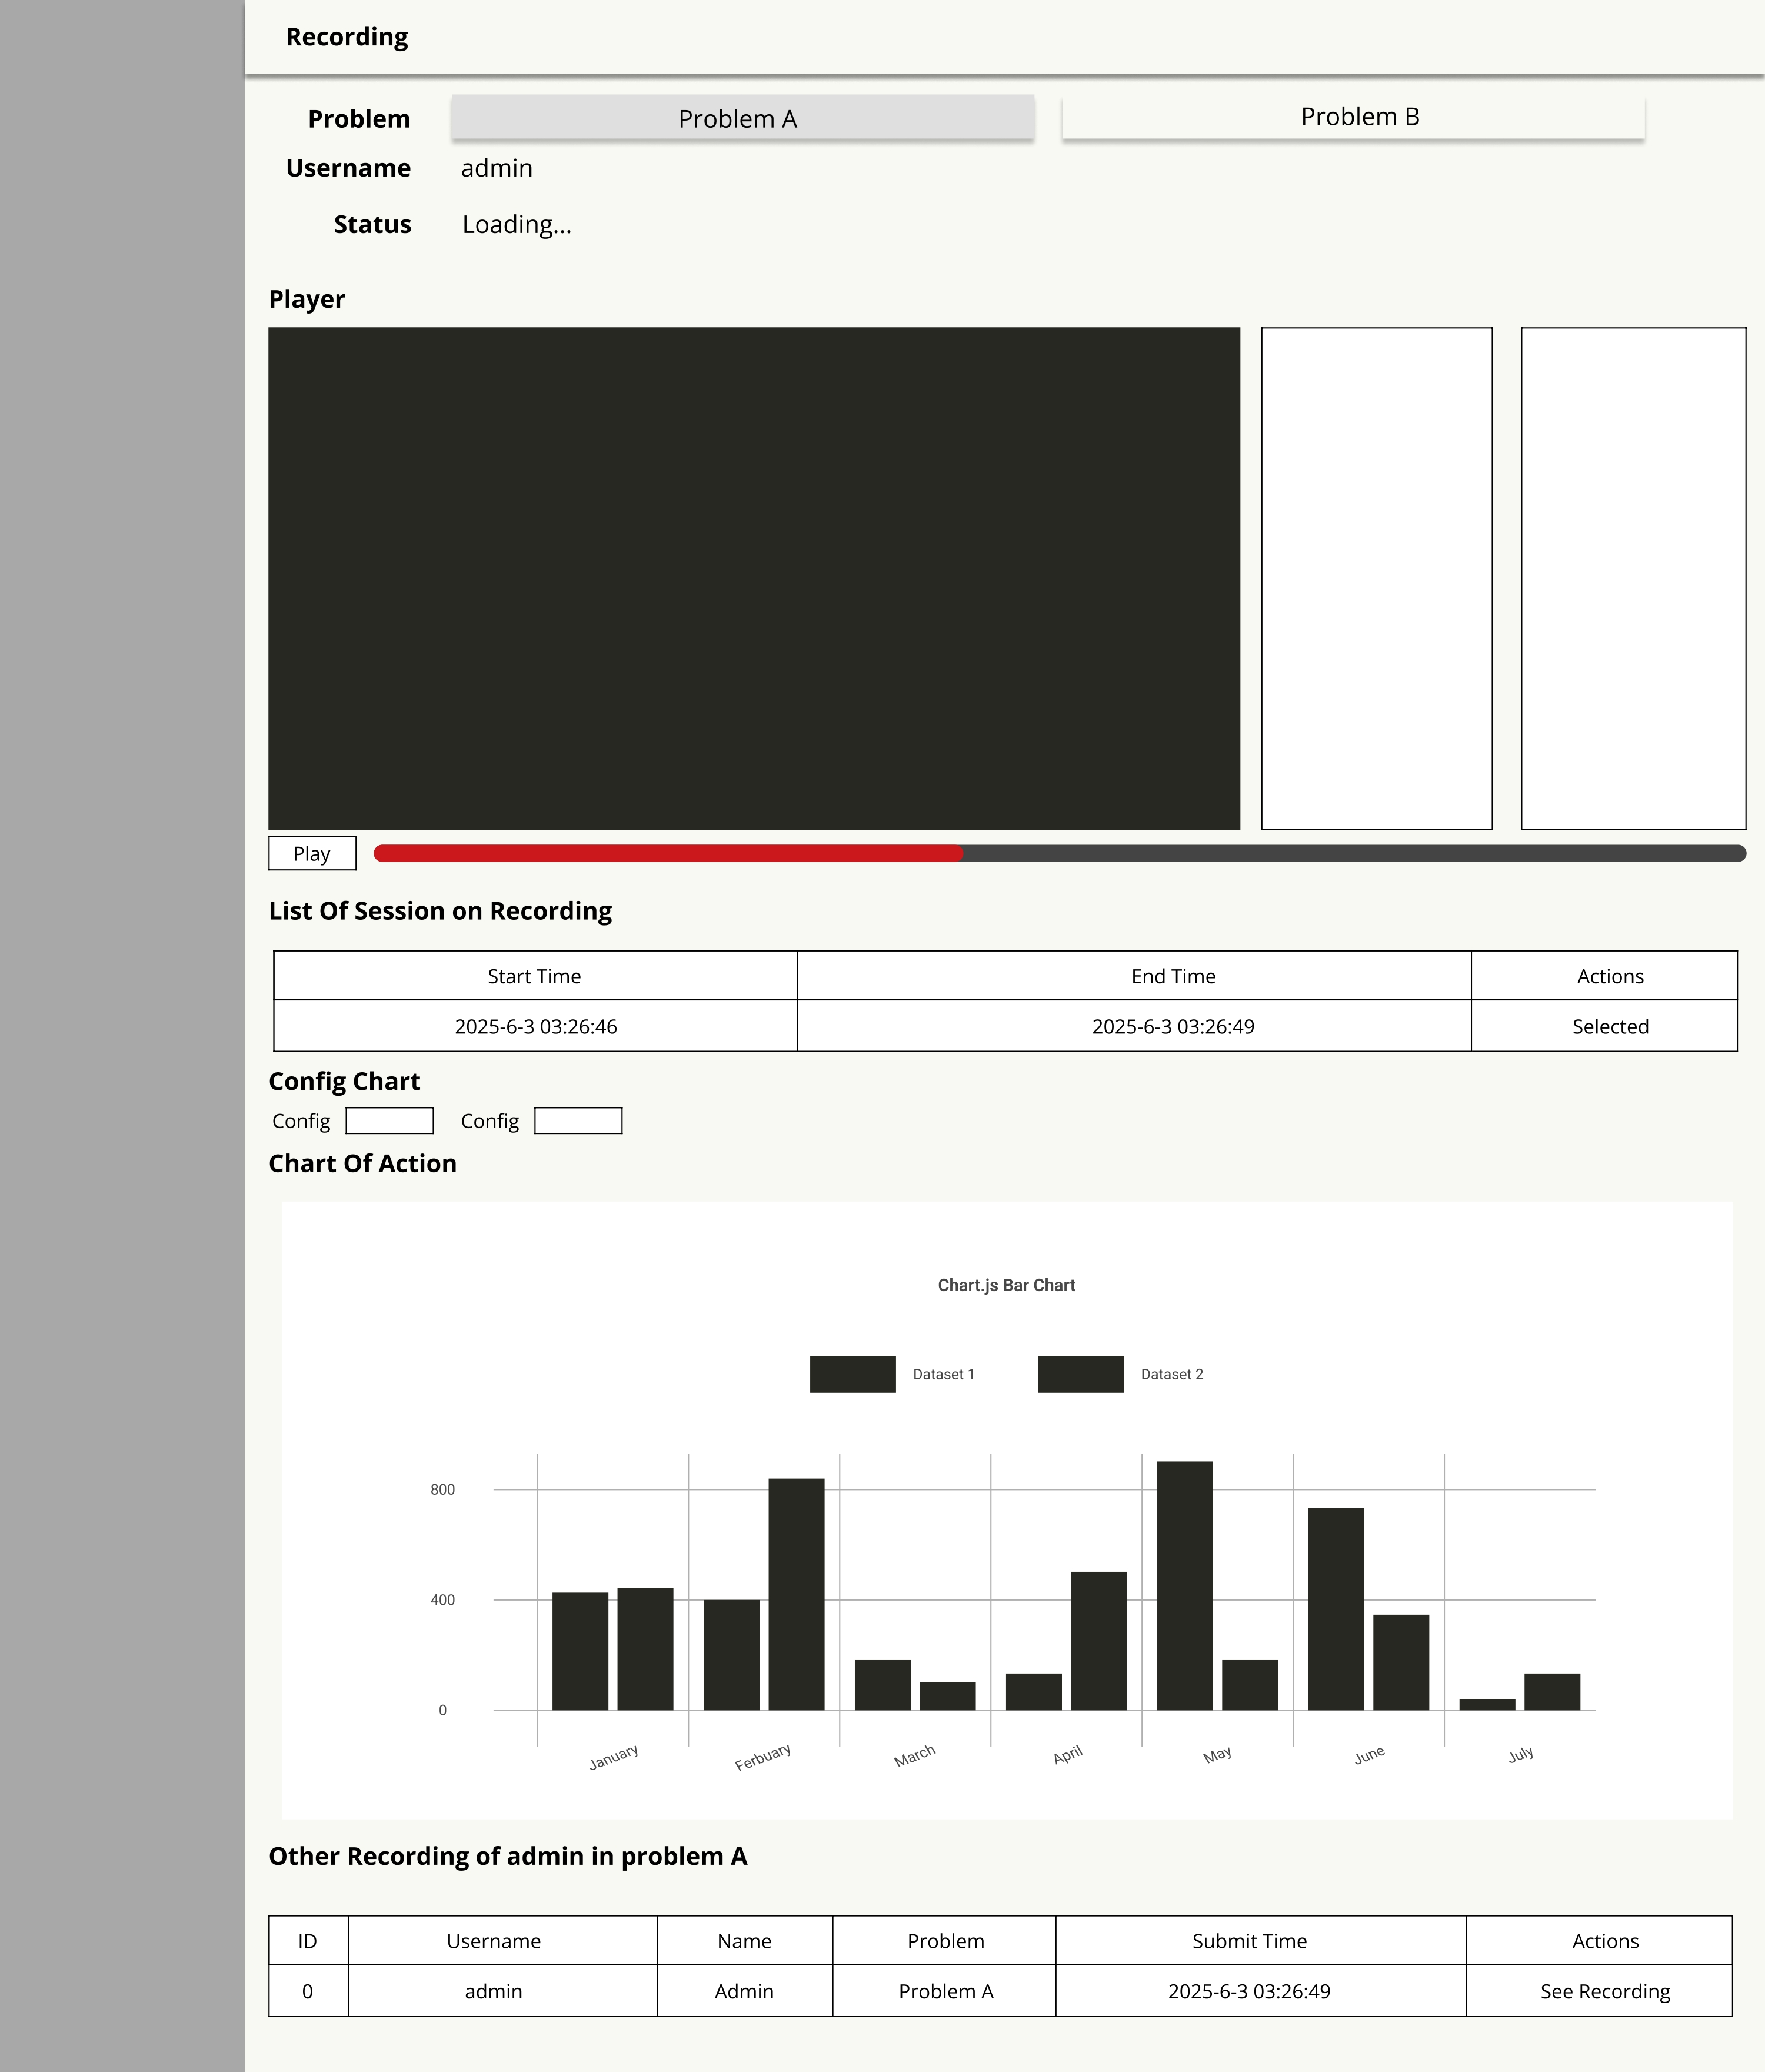
\includegraphics[width=0.75\textwidth]{design-recording.jpg}
    \caption{Rancangan Antarmuka Halaman Pemutaran Ulang}
    \label{fig:4:1:rec}
\end{figure}

\section{Rancangan Penyimpanan Rekaman}
\label{sec:4:2:storerekaman}

Rekaman yang akan disimpan akan berupa sebuah daftar \textit{event} yang terjadi. Dalam javascript, daftar tersebut akan menjadi sebuah \textit{array} yang berisi \textit{event-event} yang terjadi. Rekaman juga akan menyimpan waktu dimana rekaman dimulai, awal kode yang ada dalam editor kode dan juga awal posisi cursor dalam IDE. Maka dari itu, Rekaman akan menjadi sebuah \textit{object} javascript yang berisi sebagai berikut:

\begin{enumerate}
    \item \verb|timestart|: Waktu awal rekaman dimulai.
    \item \verb|start_value|: Isi awal dalam editor kode.
    \item \verb|start_cursor|: Posisi awal cursor dalam editor kode.
    \item \verb|events|: Daftar \textit{event} yang terjadi.
\end{enumerate}

\textit{Event} yang akan direkam juga membutuhkan beberapa data yang harus disimpan yaitu: waktu \textit{event} terjadi, \textit{event} yang terjadi, dan muatan \textit{event} yang terjadi. Maka \textit{event} juga akan disimpan dalam bentuk \textit{object} javascript. Berikut merupakan format sebuah \textit{event}:

\begin{center}
    \verb|{time: <time>, event: <event>, payload: <payload>}|
\end{center}

Berikut merupakan penjelasan tentang format penyimpanan perekaman.

\begin{itemize}
    \item \verb|<time>| akan menunjukkan pada milidetik berapa event terjadi setelah waktu awal perekaman dimulai. sedangkan \verb|<event>| dan \verb|<payload>| merupakan data event yang terjadi.
    
    \item \verb|<event>| merupakan \textit{event} yang terjadi pada waktu tersebut, pada contohnya adalah pengguna melakukan perubahan pada editor kode dengan menambahkan huruf `a', maka \textit{event} yang terjadi merupakan \textit{insert}. Semua event yang ditanggap oleh sistem akan dijelaskan pada sub Bagian \ref{sub:4:3:merekam}.
    
    \item \verb|<payload>| merupakan muatan \textit{event} yang terjadi. Muatan akan disesuaikan dengan \textit{event} yang terjadi. Sebagai contoh untuk event \textit{insert} di atas, maka isi dari \textit{event} tersebut adalah huruf `a', dan posisi cursor dalam editor kode dimana huruf tersebut dimasukkan.
\end{itemize}
    
Berikut contoh hasil untuk sebuah \textit{event insert} pada penjelasan di atas:

\begin{center}
    \verb|{time: 1203, event: "insert", payload: {data: "a", start: [10, 9]}}|
\end{center}

Penyimpanan rekaman juga akan disimpan pada folder yang sama dengan penyimpanan kode submission seperti yang dijelaskan pada Bagian \ref{sub:3:1:penyimpanankode} dengan nama file \verb|record|.

\section{Rancangan Perubahan Kode}

Untuk mengimplementasikan fitur yang diusulkan pada Bagian \ref{sec:3:sistemusulan}, diperlukannya perubahan kode berikut ini pada SharIF-Judge.

\subsection{Merekam perubahan atau event}
\label{sub:4:3:merekam}

Untuk menambahakan fitur ini, diperlukannya perubahan pada bagian javascript yaitu \verb|assets/js/|\\\verb|shj_submit.js| dalam halaman Submit. Dimana javascript tersebut akan menjalankan perekaman secara otomatis saat pengguna memilih \textit{problem} yang ada dalam \textit{assignment} yang dipilih. Berikut merupakan \textit{event} yang akan ditangkap oleh \textit{javascript} dalam halaman Submit:

\begin{itemize}
    \item Perubahan isi kode pada editor kode.
    \item Perubahan posisi cursor pada editor kode.
    \item Perubahan fokus pada web page.
    \item Pergantian \textit{tab} dalam browser.
    \item Perubahan fokus pada PDF Viewer.
    \item Perubahan isi pada editor \textit{input} dalam IDE.
    \item Perubahan isi pada editor \textit{output} dalam IDE.
    \item Aksi men-\textit{Save}.
    \item Aksi men-\textit{Save \& Execute}.
    \item Aksi men-\textit{Save \& Submit}.
\end{itemize}

\subsection{Menyimpan rekaman}
\label{sub:4:3:menyimpanrekaman}

Untuk setiap aksi menyimpan kode, menjalankan kode dengan tes kasus, dan mengumpulkan kode melalui IDE, rekaman juga akan disimpan ke dalam sistem.

Untuk menyimpan rekaman, perlu dilakukan perubahan sebagai berikut:

\begin{itemize}
    \item \textit{Controller} Submit:
        \begin{itemize}
            \item Fungsi \verb|save($type)|: \\
            Fungsi ini akan diubah agar dapat menangani data rekaman yang dikirim oleh \textit{user}. Data tersebut akan disimpan dalam folder yang sama dengan kode program.
            \item Fungsi \verb|_submit($data, $problem_id, $language, $user_dir)|: \\
            Fungsi ini akan diubah agar dapat menangani data rekaman yang dikirim oleh fungsi \verb|save($type)| dengan menambahkan parameter \verb|$rec| berisi rekaman oleh \textit{user}. Untuk setiap submit rekaman dari \textit{save-save} sebelumnya akan diubah menjadi rekaman untuk \textit{submit} tersebut.
        \end{itemize}
    \item \textit{Assets} \verb|shj_submit.js|: \\
        Menambahakan data rekaman yang dimuat ke dalam fungsi aksi menyimpan kode, menjalankan kode dengan tes kasus, dan mengumpulkan kode melalui IDE, rekaman juga akan disimpan ke dalam sistem.
\end{itemize}

\subsection{Melihat daftar rekaman}
\label{sub:4:3:melihatdaftarrekaman}

Untuk melihat semua daftar rekaman yang terjadi, maka dibutuhkannya database untuk menyimpan daftar dan mendapatkan daftar rekaman yang sudah disimpan dalam sistem. Setelah itu dibutuhkannya juga halaman baru dalam SharIF-Judge, maka perubahan \textit{Controller}, \textit{Model}, dan \textit{View} dalam SharIF-Judge.

Dikarenakan itu, perlu dilakukan perubahan kode sebagai berikut:

\begin{itemize}
    \item \textit{Controller} Submit:
    \begin{itemize}
        \item Fungsi \verb|save($type)|: \\
        Fungsi ini akan menambahkan \textit{metadata} rekaman \textit{user} ke dalam \textit{database}. \textit{Metadata} yang dimaksud adalah \textit{id problem}, \textit{id assignment}, dan \textit{user} rekaman ini direkam. Metadata dalam database digunakan untuk mendapatkan daftar rekaman yang belum disubmit pada sebuah \textit{problem} dalam \textit{assignment} beserta dengan nama \textit{user} rekaman.
        \item Fungsi \verb|_submit($data, $problem_id, $language, $user_dir)|: \\
        Fungsi ini akan menambahkan \textit{metadata} ke dalam \textit{database} sebagai daftar rekaman yang sudah di submit. \textit{Metadata} yang dimaksud adalah \textit{id problem}, \textit{id assignment}, dan \textit{user} rekaman ini direkam. Metadata dalam database digunakan untuk mendapatkan daftar rekaman yang sudah disubmit pada sebuah \textit{problem} dalam \textit{assignment} beserta dengan nama \textit{user} rekaman.
    \end{itemize}
    \item \textit{Controller} Recording: \\
    Sebuah \textit{controller} baru yang menangani segala hal mengenai sistem pemutaran ulang dalam SharIF-Judge. Fungsi yang dibutuhkan agar fitur ini berjalan hanyalah fitur untuk menunjukkan daftar rekaman dalam sistem dengan mengambil data dari \textit{model} Recording dan menaruhnya dalam \textit{view} recording. Setalah itu, \textit{controller} akan menunjukkan \textit{view} tersebut kepada \textit{user} yang sudah login dan memiliki akses \textit{instructor} atau lebih tinggi.
        % \item Fungsi \verb|index()|:
        % \item Fungsi \verb|download_record()|:
    \item \textit{Model} Recording: \\
    Sebuah \textit{model} baru yang menangani segala hal mengenai penyimpanan dan pengambilan data rekaman dalam \textit{database}. Fungsi-fungsi yang direncanakan dalam \textit{model} adalah sebagai berikut:
    \begin{itemize}
        \item Fungsi \verb|get_recording()|: \\
        Fungsi ini digunakan untuk mendapatkan seluruh daftar rekaman dalam database, fungsi ini juga dapat menyaring daftar rekaman berdasarkan \textit{assignment}, \textit{problem}, dan \textit{user}.
        \item Fungsi \verb|add_recording()|: \\
        Fungsi ini digunakan untuk menaruh sebuah rekaman ke dalam database.
    \end{itemize}
    \item \textit{View} \verb|Recording_list|: \\
    Sebuah \textit{view} baru yang menampilkan daftar rekaman yang ada dalam sistem. \textit{View} ini akan digunakan oleh \textit{Controller} Recording.
\end{itemize}

\subsection{Pemutaran ulang rekaman}

Untuk dapat memutar ulang rekaman diperlukan beberapa perubahan kode dalam SharIF-Judge. Berikut merupakan rencana perubahan kode dalam SharIF-Judge:

\begin{itemize}
    \item \textit{Controller} Recording: \\
    Sebuah \textit{controller} baru yang menangani segala hal mengenai sistem pemutaran ulang dalam SharIF-Judge. Untuk fitur pemutaran ulang rekaman, diperlukan dua fungsi pada \textit{controller} yaitu sebagai berikut:
    \begin{itemize}
        \item Fungsi \verb|index()|: \\
        Fungsi ini digunakan untuk menunjukkan \textit{view} \verb|Recording| kepada \textit{user}.
        \item Fungsi \verb|download_record()|: \\
        Fungsi ini digunakan untuk mendapatkan file rekaman dalam sistem. Fungsi ini akan dipanggil mengunakan AJAX dalam \textit{assets} \verb|Recording.js|.
    \end{itemize} 
    \item \textit{Model} Recording: \\
    Sebuah \textit{model} baru yang menangani segala hal mengenai penyimpanan dan pengambilan data rekaman dalam \textit{database}. Fungsi yang dibutuhkan oleh fitur pemutaran ulang rekaman adalah fungsi \verb|get_recording()| untuk mendapatkan seluruh daftar rekaman sebuah \textit{user} dalam database berdasarkan \textit{problem} dan \textit{assignment}.
    \item \textit{View} \verb|Recording|: \\
    Sebuah \textit{view} baru yang menampilkan rekaman sebuah \textit{user} yang ada dalam sistem. \textit{View} ini akan digunakan oleh \textit{Controller} Recording.
    \item \textit{Assets} \verb|Recording.js|: \\
    Sebuah \textit{assets} javascript yang digunakan oleh \textit{view} \verb|Recording| sebagai \textit{script} yang akan dijalankan oleh \textit{browser user}.
\end{itemize}